\section{Правила игры}

\subsection{Игровой набор}

Для игры используются 136 специальных костей, которые чаще называют \textit{тайлами}. Есть 34 вида тайлов, и каждый из них встречается в наборе ровно четыре раза (34 х 4 = 136). На одной стороне тайла находится значимое изображение, другая же, рубашка, у всех тайлов одинакова.

Тайлы мастей:

\begin{tabular}{ |C{3.5cm}|c|c|c|c|c|c|c|c|c| } 
	\hline
	Масть/номинал & 1 & 2 & 3 & 4 & 5 & 6 & 7 & 8 & 9 \\
	\hline
	Ман \newline & \mahjong{1m} & \mahjong{2m} & \mahjong{3m} & \mahjong{4m} & \mahjong{5m} & \mahjong{6m} & \mahjong{7m} & \mahjong{8m} & \mahjong{9m} \rule[1ex]{0pt}{5ex} \\
	\hline
	Пин \newline & \mahjong{1p} & \mahjong{2p} & \mahjong{3p} & \mahjong{4p} & \mahjong{5p} & \mahjong{6p} & \mahjong{7p} & \mahjong{8p} & \mahjong{9p} \rule[1ex]{0pt}{5ex} \\
	\hline
	Соу \newline & \mahjong{1s} & \mahjong{2s} & \mahjong{3s} & \mahjong{4s} & \mahjong{5s} & \mahjong{6s} & \mahjong{7s} & \mahjong{8s} & \mahjong{9s} \rule[1ex]{0pt}{5ex} \\
	\hline
	Японское чтение & ии & рян & сан & суу & уу & ро & чии & паа & чуу \\
	\hline 
\end{tabular}


Благородные тайлы (обратите внимание, порядок важен):

\begin{tabular}{ |c|C{2cm}|C{2cm}|C{2cm}|C{2cm}| } 
	\hline
	 \rule[0ex]{0pt}{6ex} Ветра & \mahjong{1z} \newline Восток & \mahjong{2z} \newline Юг & \mahjong{3z} \newline Запад & {\mahjong{4z} \newline Север} \\
	\hline
	Японское чтение & тон & нан & ся & пей \\
	\hline
\end{tabular}

\begin{tabular}{ |c|C{2cm}|C{2cm}|C{2cm}| } 
	\hline
	 \rule[0ex]{0pt}{6ex} Драконы & \mahjong{5z} \newline Белый & \mahjong{6z} \newline Зеленый & \mahjong{7z} \newline Красный \\
	\hline
	Японское чтение & хаку & хацу & чун \\
	\hline
\end{tabular}

Для подсчета очков в игре используются палочки следующих номиналов:

\begin{tabular}{ |c|c|c| } 
	\hline
	
\includegraphics{tenbo10000} & 10000 очков & x1 \\
	
\includegraphics{tenbo5000} & 5000 очков & x2 \\
	
\includegraphics{tenbo1000} & 1000 очков & x9 \\
	
\includegraphics{tenbo100} & 100 очков & x10 \\
	\hline
\end{tabular}

Иногда можно встретить в наборах палочки номиналом 500 очков, как правило они выглядят так же как палочки на 100 очков, но окрашенные в зеленый цвет.

Общее количество очков в начале игры у каждого игрока равно 30000. Количество палочек в наборе может также отличаться, например может быть три палочки по 5000 и четыре по 1000, главное чтобы общее количество соответствовало указанному.

\pagebreak

Также в игре используются:
\begin{itemize}
	\item Индикатор первого дилера - небольшая пластинка с изображением восточного ветра (\textnihon{東}) с одной стороны и южного ветра (\textnihon{南}) с другой;
	\item Два шестигранных кубика с цифрами от 1 до 6.
\end{itemize}

\subsection{Подготовка к игре}

В риичи-маджонг играют вчетвером. Для игры используют небольшой квадратный стол (~75х75 см), с каждой стороны которого садится по игроку. Каждому месту за столом присваивается условная сторона света, и расположены они в порядке тайлов ветров против часовой стрелки: восток (\textnihon{東}), юг (\textnihon{南}), запад (\textnihon{西}), север (\textnihon{北}), т. е. порядок «неправильный» и отличается от настоящего расположения сторон на карте мира\footnote{Порядок ветров соответствует расположению сторон света на карте звездного неба.}. Выбор мест производится по договорённости или по жребию. Способ распределения мест таков: на стол кладутся четыре разных тайла ветров рубашкой вверх, игроки вытягивают их по очереди, и каждый занимает соответствующее место. Ветер, соответствующий месту игрока, называется \textit{ветром места}. 

Игрок, вытянувший восток, занимает в игре особое положение \textit{дилера}. Рядом с ним в начале игры кладётся индикатор первого дилера. Обычно дилер выбирает место за столом, остальные рассаживаются относительно него согласно вытянутым ветрам.

Игра делится на раунды, также названные по сторонам света – восточный (первый) и южный (второй), и раздачи. Существует два варианта партий: короткая игра, где играется только восточный раунд, называется \textit{тонпусен}, длинная и с восточным, и с южным – \textit{ханчан}. Ветер, соответствующий текущему раунду, называется \textit{ветром раунда}. Раунд по умолчанию состоит из четырёх раздач (хотя в отдельных случаях, оговорённых правилами, могут назначаться дополнительные раздачи), и каждую новую раздачу происходит сдвиг сторон света за столом на одно место против часовой стрелки: игрок, в первой раздаче бывший на юге, во второй оказывается дилером, в третьей – севером и т. д, сами игроки при этом не пересаживаются. Таким образом, смена раунда происходит, когда дилерство возвращается к игроку, бывшему дилером в первой раздаче. Индикатор первого дилера всё время остаётся лежать рядом с дилером первой раздачи; во время восточного раунда он повёрнут вверх стороной, где нарисован иероглиф востока, а с началом южного переворачивается. Для указания на дилера текущей раздачи с его стороны стола после подготовки к раздаче кладутся кубики.

Перед началом каждой раздачи игроки кладут все тайлы на стол рубашкой вверх и тщательно их перемешивают. После этого каждый игрок строит перед собой «стену» высотой в 2, шириной в 1 и длиной в 17 тайлов рубашкой вверх, размещая её так, чтобы в итоге четыре участка стены от разных игроков образовали замкнутый квадрат. Затем дилер бросает кубики и отсчитывает против часовой стрелки столько сторон квадрата, сколько выпало на кубиках суммарно, начиная со своей стороны (на рис.1 показан пример для выпавшей суммы 8).

\begin{figure}[H]
	\centering
	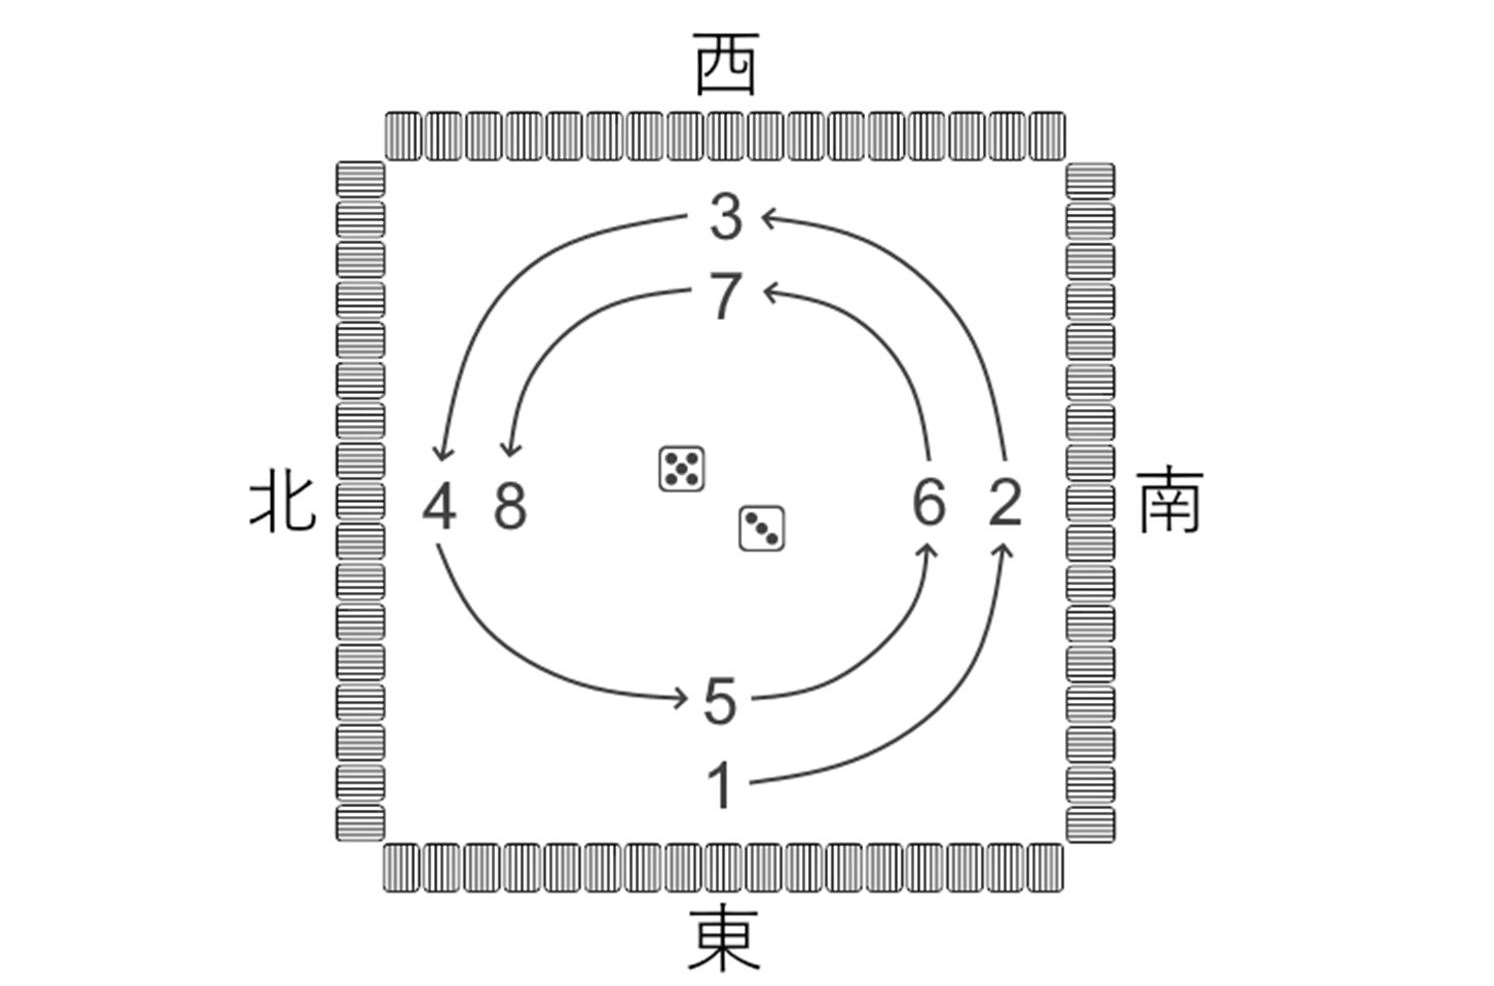
\includegraphics[width=16cm]{table-deal-start.png}
	\caption{Определение разлома стены}
\end{figure}

Затем игрок, на чью сторону указал дилер (в примере выше – север) отсчитывает от правого конца своей стороны стены столько тайлов, какое число выпало на кубиках до этого (в примере – 8) и немного отодвигает их от соседних тайлов вправо, создавая разлом стены. После этого он отсчитывает от разлома в обратную сторону 7 тайлов и делает второй разлом, обособляя получившуюся группу из 14 тайлов (см. рис.2). Эта группа называется мёртвой стеной и не разбирается в процессе игры. Оставшаяся часть стены называется живой стеной и используется во время раздачи для получения игроками тайлов (наподобие колоды карт). Разбирается она стопками верхний-нижний по часовой стрелке, начиная с верхнего тайла первой стопки после разлома и заканчивая нижним последней перед мёртвой стеной. Стена считается непрерывной, и переход через углы не имеет никакого значения как при формировании мёртвой стены, так и при последующем разборе.

Третий верхний тайл от конца мёртвой стены переворачивается рубашкой вниз (на рисунке это 6 ман) и служит в данной раздаче индикатором доры – тайла, дающего дополнительные очки при его наличии в руке. Подробно о дорах и принципе работы индикаторов рассказано в разделе VIII.

\begin{figure}[H]
	\centering
	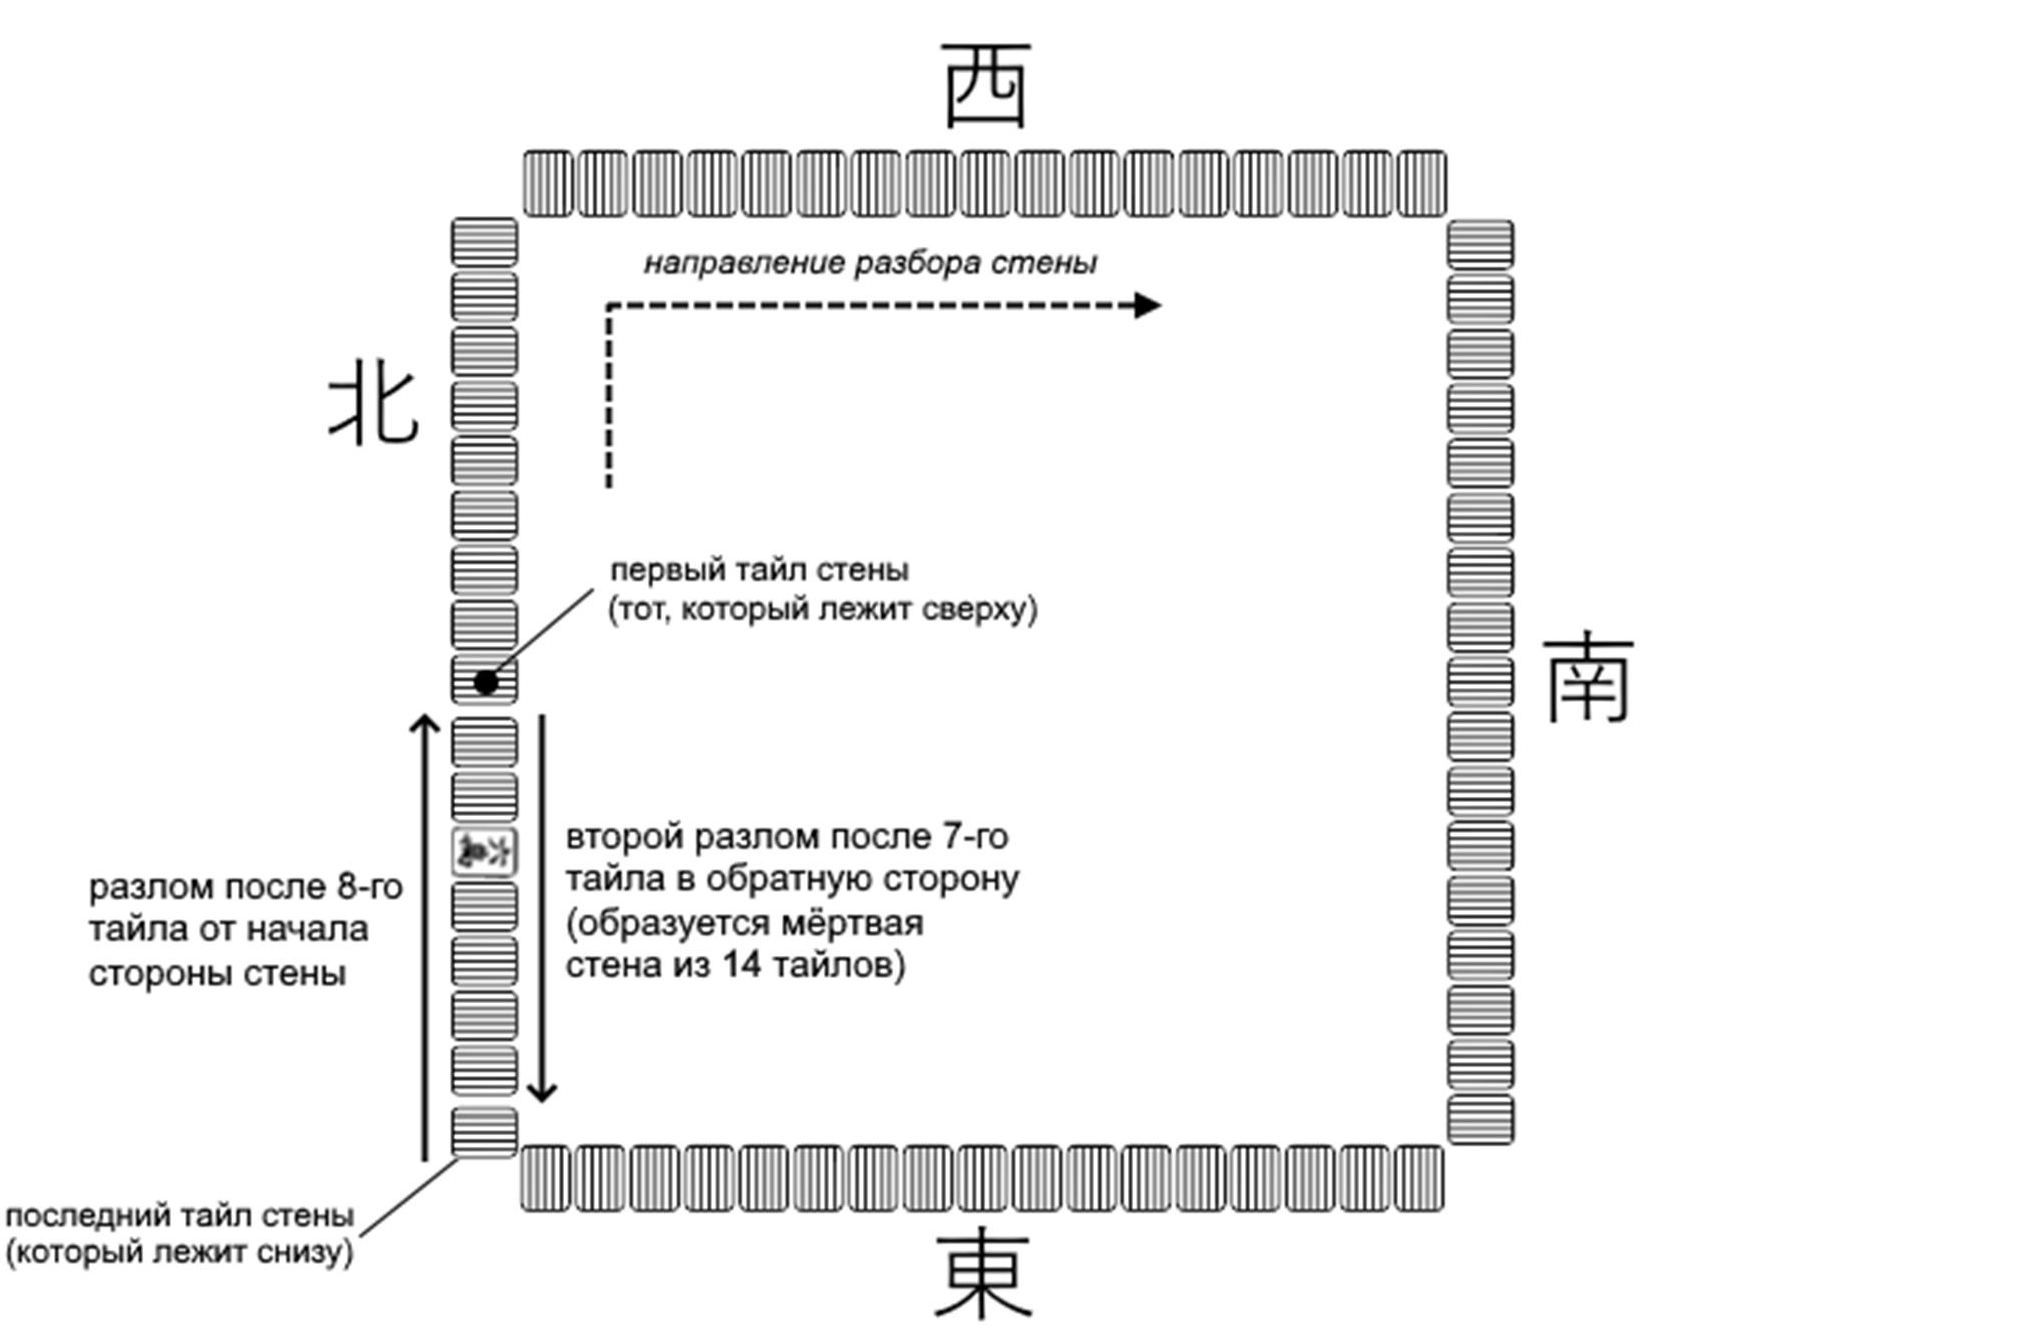
\includegraphics[width=16cm]{table-deal-start-2.png}
	\caption{Мертвая и живая стены}
\end{figure}

После открытия индикатора доры игроки берут себе со стены тайлы в стартовые руки. Начиная с дилера по очереди против часовой стрелки игроки начинают брать от начала живой стены по четыре тайла (две стопки по 2), пока у каждого не окажется 12 тайлов. После этого игроки в том же порядке берут ещё по одному тайлу (порядок разбора – всегда от верхнего к нижнему), а затем дилер берёт себе ещё один тайл (см. рис.3). Таким образом, в начале раздачи дилер имеет 14 тайлов, а остальные – по 13. Тайлы своих рук игроки расставляют перед собой в ряд вертикально изображением к себе, так, чтобы остальные видели только их рубашки. Для удобства игроки сортируют руки: ставят рядом тайлы одной масти по порядку номеров и одинаковые благородные тайлы. Допустим, игрок взял себе в стартовую руку следующие тайлы:

\mahjong{5m 6s 4m 8s 3z 9m 7z 2z 1s 3m 7z 7s 4m}

Он может отсортировать их следующим образом:

\mahjong{1s 678s 34459m 2377z}

Разные масти могут быть отсортированы слева направо или справа налево, а разные благородные тайлы могут стоять в разных местах – всё зависит от удобства для игрока и времени, затрачиваемого на сортировку. В данном описании правил в дальнейшем для простоты все руки будут показаны отсортированными одинаково: ман, пин, соу слева направо, ветра по порядку, драконы по порядку.

В компьютерном маджонге построение стены, её разлом, набор и сортировка стартовых рук как правило происходят автоматически, и когда начинается раздача игроки сразу же видят свои отсортированные стартовые руки и индикатор доры. 

\begin{figure}[H]
	\centering
	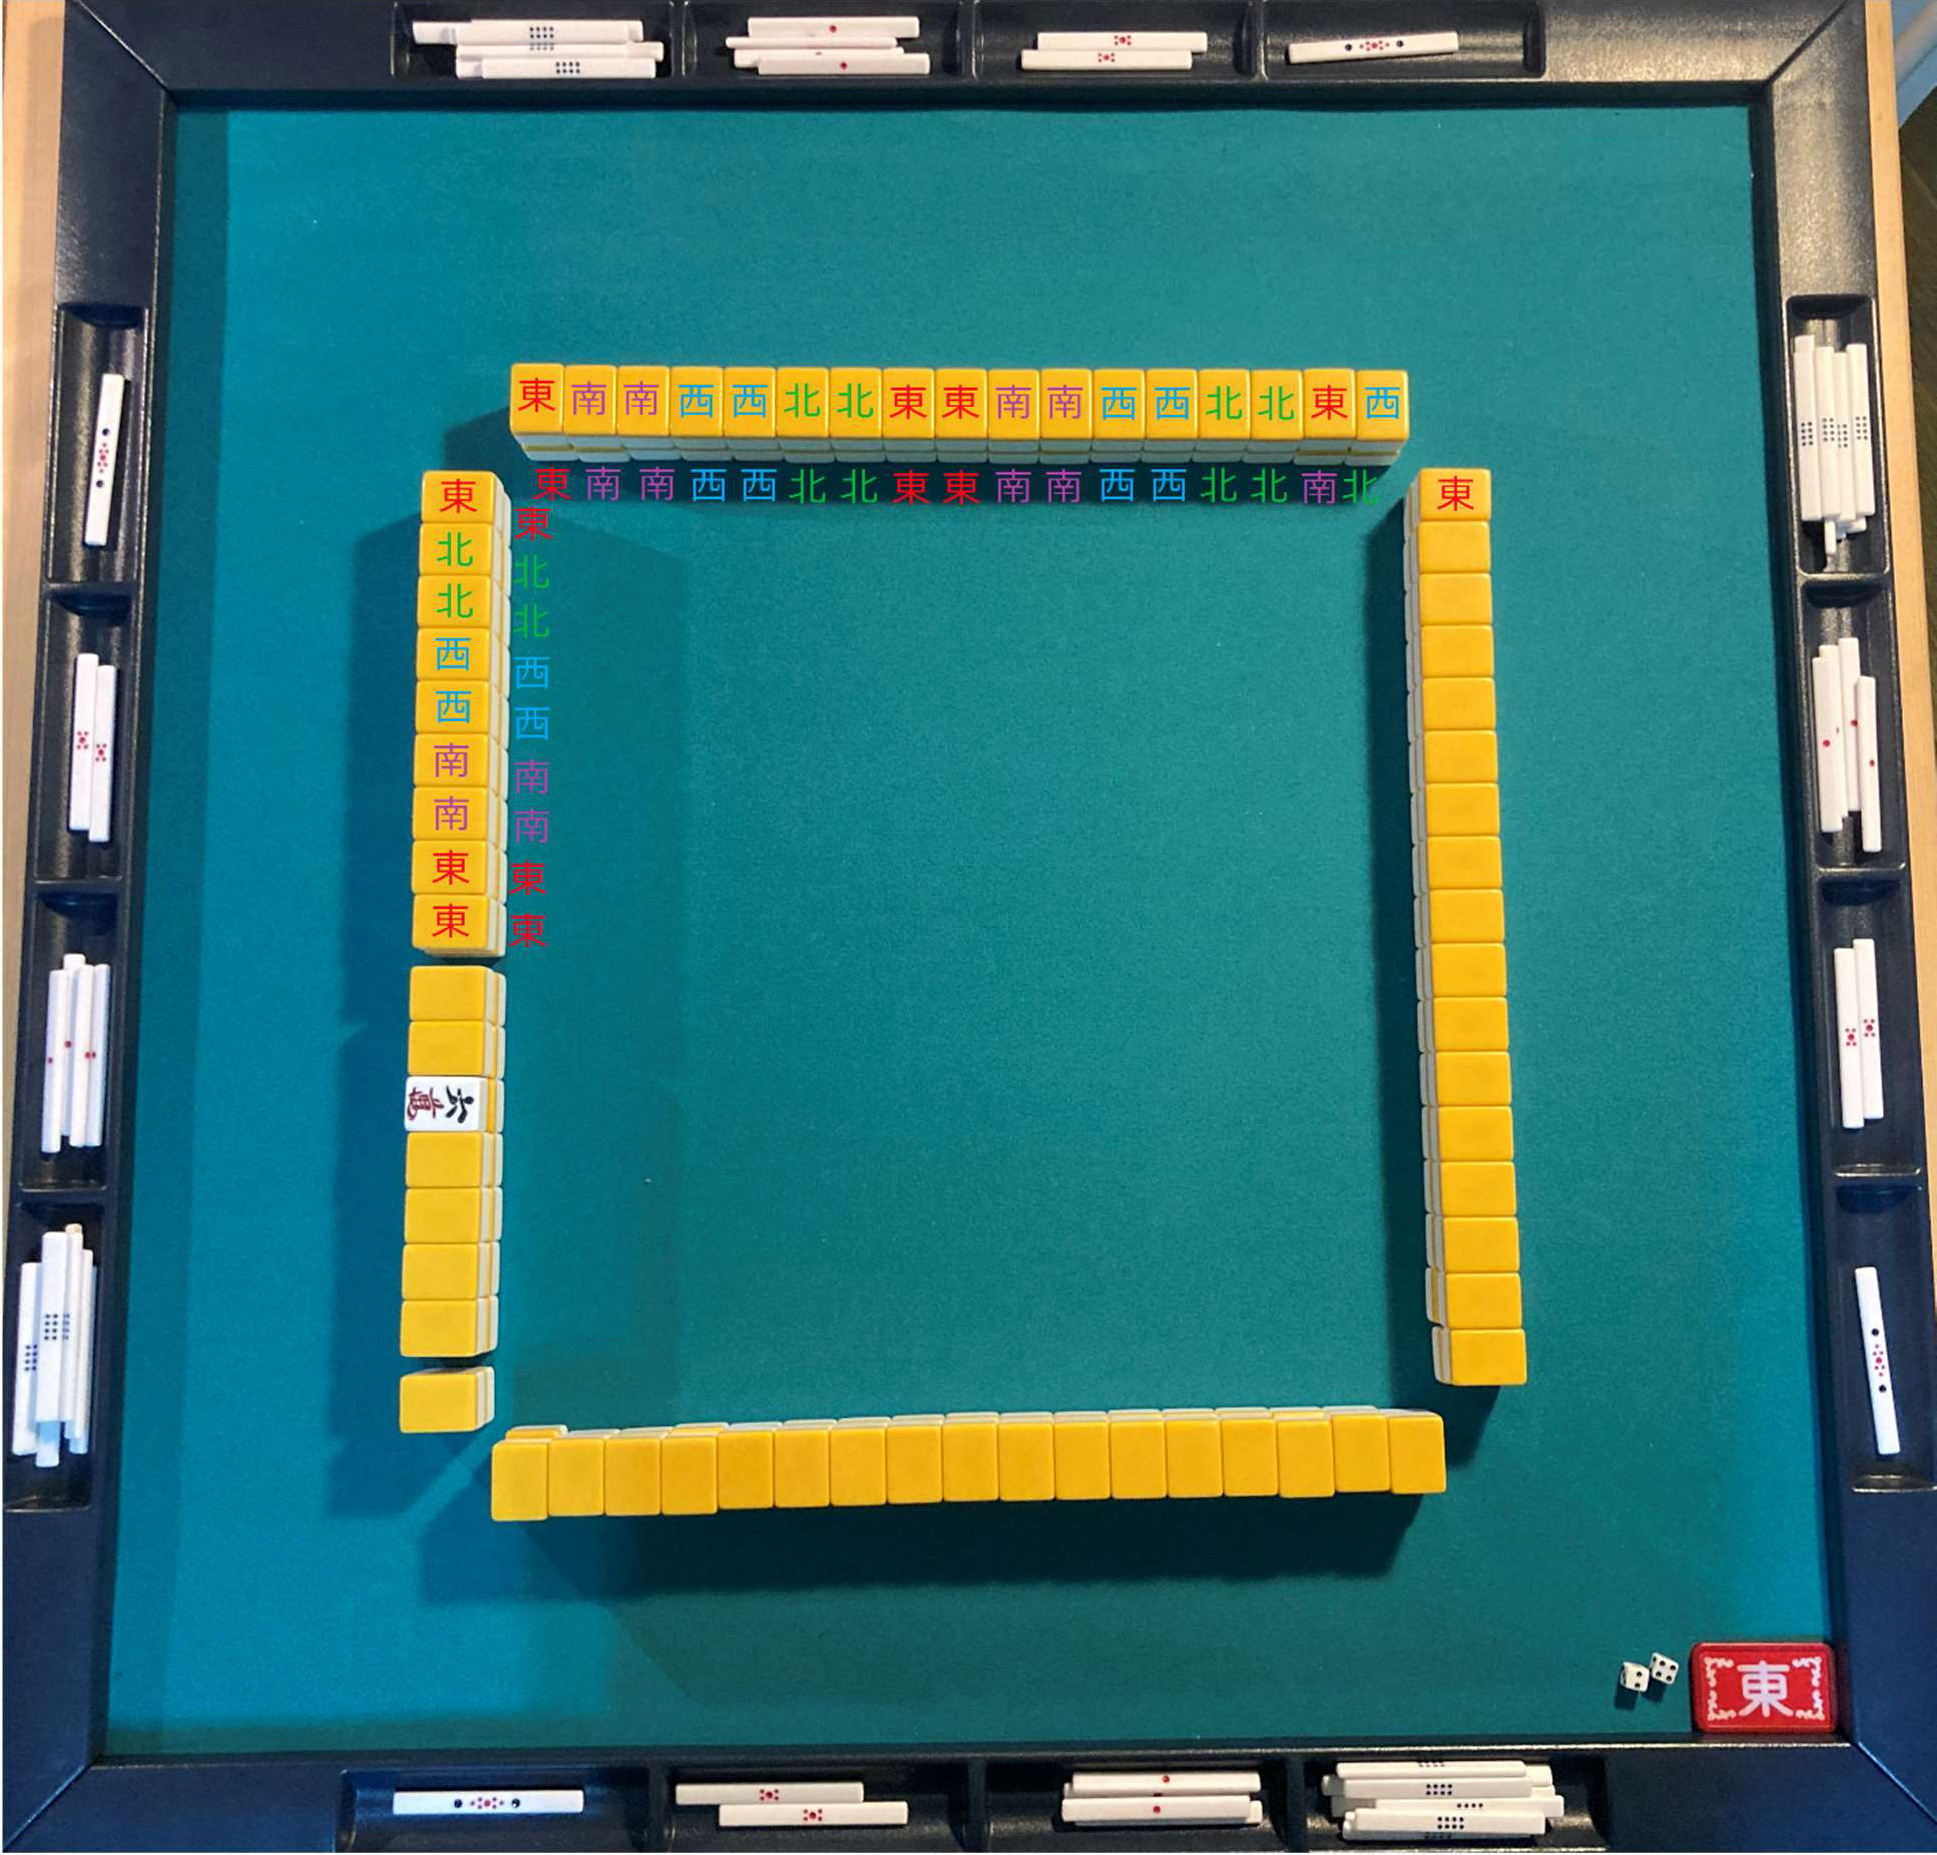
\includegraphics[width=16cm]{table-deal-start-3.png}
	\caption{Порядок разбора стены, фото}
\end{figure}

Обратите внимание на подписи тайлов - они показывают, какой игрок должен их взять (верхние тайлы стены подписаны прямо на рубашке, нижние – рядом). Предположим, что сейчас идёт первая раздача восточного раунда: индикатор первого дилера повёрнут иероглифом востока кверху, а кубики как индикатор текущего дилера лежат рядом с ним, т. е. первый дилер является дилером в этой раздаче.

\section{Ход раздачи}

В ходе раздачи, которая начинается сразу же после набора и сортировки всеми стартовых рук, игроки изменяют состав своих рук, набирая в них по одному новые тайлы с живой стены и выбрасывая ненужные. Цель каждого игрока в раздаче – собрать в руке четыре сета и одну пару (два одинаковых тайла). При объявлении кем-либо победы с готовой рукой раздача заканчивается. Цель всей игры – набрать как можно больше очков, получаемых в основном за собранные руки.

Сет – это определённая комбинация из трёх или четырёх тайлов. Они бывают трёх видов:
\begin{itemize}
	\item Три одинаковых тайла - \textit{пон};
	\item Четыре одинаковых тайла – \textit{кан};
	\item Последовательность из трёх тайлов одной масти подряд (по типу 1-2-3, 3-4-5 и т. п.) – \textit{чи}. Последовательности можно собирать только из тайлов мастей, и в них не должно быть перехода через девятку: 8-9-1 и 9-1-2 не засчитываются как чи.
\end{itemize}

Один тайл не может одновременно входить в два сета. В примере ниже в руке уже есть готовый пон из 4 ман, чи 7-8-9 ман и пара красных драконов, но последовательность 3-4-5-6-7 пин не засчитывается за два чи: для завершения этой формы в два сета требуется получить ещё один тайл (2, 5 либо 8 пин).

\mahjong{444789m 34567p 77z}

В руке из примера выше 13 тайлов, как и в любой руке не-дилера в начале раздачи, но выигрышная рука должна содержать как минимум 14 тайлов (3+3+3+3+2, если же в руке есть каны, число тайлов может доходить до 18). Четырнадцатый тайл игроки получают в свои ходы во время раздачи: раздача начинается с хода дилера, который сбрасывает из руки один из своих 14 тайлов, кладя его рубашкой вниз в центр стола; затем ход переходит к следующему игроку против часовой стрелки, который берёт первый тайл из оставшейся части живой стены и также сбрасывает один тайл из своей руки (можно сбрасывать и тайл, только что взятый со стены – такой сброс называется \textit{цумогири}). Затем ход переходит к следующему игроку, и так раздача продолжается до тех пор, пока кто-либо не соберёт руку и объявит победу, или же пока в живой стене не закончатся тайлы. 

Ходы в риичи-маджонге обязательны, пропускать взятие со стены либо сброс нельзя. Каны, а вместе с ними и руки, содержащие более 14 тайлов, возможно образовать специальными объявлениями, о которых рассказывается в следующем разделе. Ходы четырёх игроков, начиная от дилера, образуют круг раздачи. После окончания круга ход вновь переходит к дилеру, и начинается следующий круг. Группы сброшенных тайлов в центре стола называются сбросами или \textit{дискардами}. Каждый игрок имеет свой отдельный дискард. Тайлы следует выкладывать в сброс слева направо тремя рядами по 6 штук (начиная с ближнего к центру стола и далее по направлению к себе); четвёртый же ряд чаще не начинают, а вместо этого продолжают третий.

\begin{figure}[H]
	\centering
	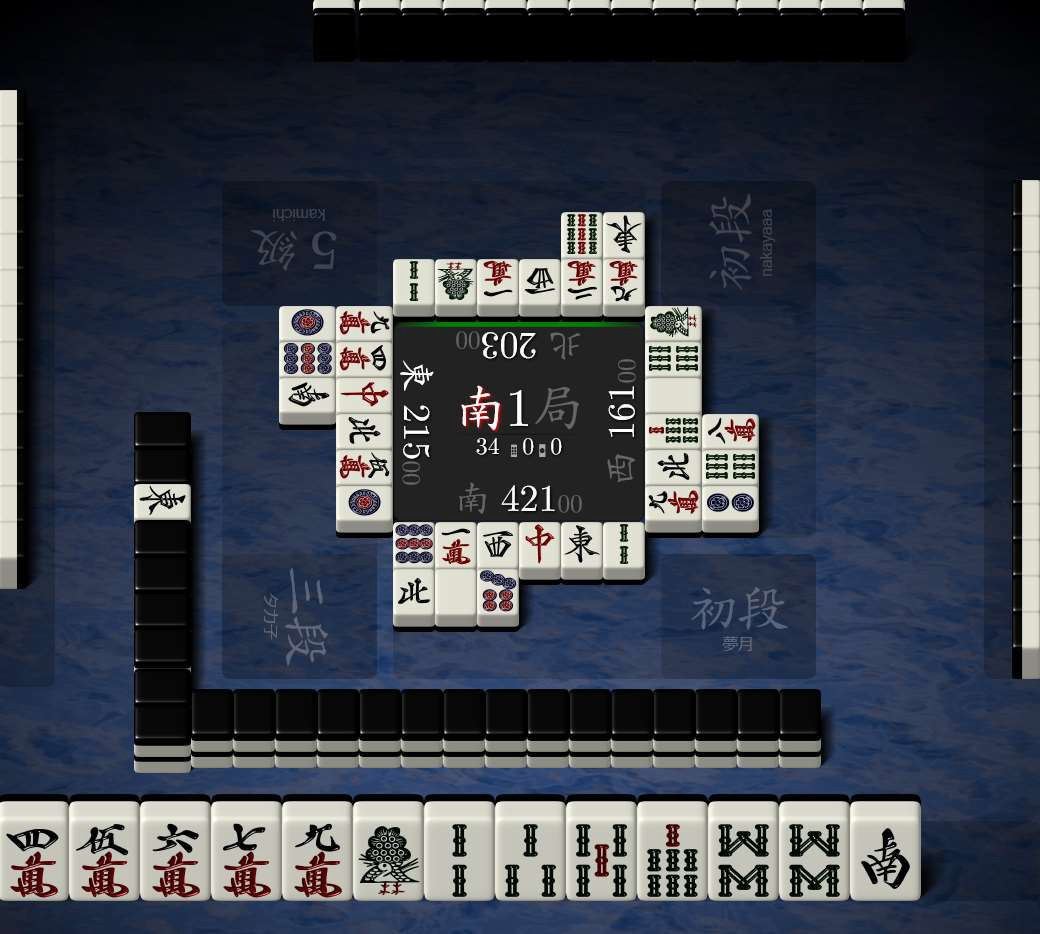
\includegraphics[width=16cm]{tenhou-deal.jpg}
	\caption{Пример раздачи на сервере tenhou.net}
\end{figure}

Рассмотрим вид стола в процессе раздачи на онлайн-сервере tenhou.net (рис.4). В центре – указатель раунда и номера раздачи за раунд (южный, первая) и указатели мест игроков со счётчиками очков (мы юг с 42100 очков; на онлайн-серверах вместо палочек используются цифровые счётчики). Вокруг центра – дискарды игроков, ниже – живая стена, слева – мёртвая стена с индикатором доры восточным ветром. По краям стола расположены руки игроков. Сейчас 9-й круг, ход севера: он получил тайл со стены, но ещё не совершил сброс. Пришедший со стены тайл сначала ставят отдельно (здесь он стоит слева от основной руки, если смотреть от нас), и встраивают в руку только после сброса, если сброшен другой тайл.

\section{Объявления в игре}

% TODO: Сорокин

\section{Фуритен и временный фуритен}

Правило \textit{фуритен} (\textnihon{フリテン}), или правило упущенного сброса, запрещает игроку объявлять рон, если хоть один из выигрышных тайлов, завершающих руку, лежит у него в дискарде. При этом как дискард учитываются и тайлы, взятые оттуда для сетов другими игроками. Именно из-за этого при объявлениях сетов требуется указывать какой тайл был взят и с кого из противников, кладя один из тайлов боком с соответствующей стороны.

Например, рассмотрим игрока со следующей рукой:

\mahjong{33456678m 23p 678s}

Предположим, дискард у игрока следующий:

\mahjong{1p 4z 7z 2s 4s 9m}

В данном случае игрок не может объявить рон ни при сбросе противником 1 пин, ни при сбросе 4 пин, потому что в его дискарде есть «упущенный» выигрышный тайл 1 пин. При этом ограничений на объявление цумо нет. Если игрок перестроит свою руку так, чтобы сброшенные в дискард тайлы не завершали выигрышное ожидание, фуритен перестанет действовать, и он снова сможет объявлять рон. Например, это будет возможно если руку выше изменить следующим образом взятием 5 пин и сбросом 2 пин: 

\mahjong{33456678m 35p 678s}

В этом случае ожидание на 1 пин пропадёт, и игрок сможет объявить рон на сброшенную кем-либо 4 пин. 

Фуритен даёт возможность для игры в защиту: тайлы, лежащие в сбросе у противника, можно уверенно сбрасывать, не опасаясь, что он объявит на них рон (при победе по рону игрок получает очки за счёт сбросившего выигрышный тайл; о выплатах см. раздел IX). Есть и более продвинутые приёмы защиты, основанные на фуритене, которым посвящены отдельные специализированные статьи, в данном руководстве не рассматриваемые.

\textit{Временный фуритен} – это отдельное правило, которое не позволяет игроку объявлять рон, если на текущем круге считая от хода игрока уже был сброшен какой-либо из выигрышных для него тайлов. Действие временного фуритена заканчивается с первым же ходом игрока – в момент, когда игрок формально может сменить ожидание. Допустим у нас на нашем ходу имеется следующая рука:

\mahjong{123456789m 99s 11z}

В случае если игрок справа сбросил 9 со и мы пропустили возможный рон, а сразу за ним игрок напротив сбрасывает восток или ещё одну 9 со, объявлять рон на этот тайл нельзя, потому что на этом круге рон уже был пропущен. Если же кто-то ещё раз сбросит 9 со или восток уже после следующего нашего хода, рон объявить будет можно.

Временный фуритен существует для предотвращения избирательности в объявлении рона, но иногда действует во вред игрокам в темпае, если после одного пропущенного выигрышного тайла на том же круге сбрасывается тайл, дающий руке большую стоимость, чем первый. Если игрок пропустил один рон после объявления риичи, из-за временного фуритена он не может победить по рону до конца раздачи, т. к. после риичи сменить ожидание невозможно (подробно о риичи рассказывается в посвящённом ему разделе VII).
